\documentclass[a4paper, 12pt]{article} % classe de base
\usepackage[utf8]{inputenc} % générer .bib avec zotero, encodage europe centrale 8859 2
\usepackage[american]{babel}	%
\usepackage{amsfonts,amssymb}
\usepackage{url}	
\usepackage{fancyhdr} 
\usepackage{multirow}
\usepackage{appendix}                                      
\usepackage{perpage}			
\usepackage[pdftex]{color,graphicx,graphics,epsfig}
\usepackage[square]{natbib} 
\graphicspath{{Images/}}
\usepackage{float}
\usepackage{amsmath} 
%\usepackage[hyper=true,toc=true,number=none,style=list]{glossary}
\usepackage[colorlinks=true]{hyperref} 
\hypersetup{urlcolor=blue,linkcolor=black,citecolor=red} 
\usepackage{setspace}
\usepackage{pdfpages}
\usepackage{listings}
\usepackage{xcolor}
\usepackage{subcaption}
 
\usepackage{fixmath}

\usepackage{listings}

\usepackage{color}
\definecolor{gray}{rgb}{0.4,0.4,0.4}
\definecolor{darkblue}{rgb}{0.0,0.0,0.6}
\definecolor{cyan}{rgb}{0.0,0.6,0.6}

\lstset{
	basicstyle=\ttfamily,
	columns=fullflexible,
	showstringspaces=false,
	commentstyle=\color{gray}\upshape
}

\lstdefinelanguage{XML}
{
	morestring=[b]",
	morestring=[s]{>}{<},
	morecomment=[s]{<?}{?>},
	stringstyle=\color{black},
	identifierstyle=\color{darkblue},
	keywordstyle=\color{cyan},
	morekeywords={xmlns,version,type}% list your attributes here
}


\newcommand\crule[3][black]{\textcolor{#1}{\rule{#2}{#3}}}

\definecolor{cl1}{RGB}{123,239,77}
\definecolor{cl2}{RGB}{255,5,1}
\definecolor{cl3}{RGB}{19,29,222}
\definecolor{cl4}{RGB}{152,16,25}
\definecolor{cl5}{RGB}{228,239,8}
\definecolor{cl6}{RGB}{239,173,29}

\definecolor{cl21}{RGB}{167,93,185}
\definecolor{cl22}{RGB}{255,5,1}
\definecolor{cl41}{RGB}{58,31,15}
\definecolor{cl42}{RGB}{152,16,25}
\definecolor{cl43}{RGB}{72,6,73}


%\usepackage{listingsutf8}
\lstset{
	literate=%
	{á}{{\'a}}1
	{í}{{\'i}}1
	{é}{{\'e}}1
	{ý}{{\'y}}1
	{ú}{{\'u}}1
	{ó}{{\'o}}1
	{ě}{{\v{e}}}1
	{š}{{\v{s}}}1
	{č}{{\v{c}}}1
	{ř}{{\v{r}}}1
	{ž}{{\v{z}}}1
	{ď}{{\v{d}}}1
	{ť}{{\v{t}}}1
	{ň}{{\v{n}}}1                
	{ů}{{\r{u}}}1
	{Á}{{\'A}}1
	{Í}{{\'I}}1
	{É}{{\'E}}1
	{Ý}{{\'Y}}1
	{Ú}{{\'U}}1
	{Ó}{{\'O}}1
	{Ě}{{\v{E}}}1
	{Š}{{\v{S}}}1
	{Č}{{\v{C}}}1
	{Ř}{{\v{R}}}1
	{Ž}{{\v{Z}}}1
	{Ď}{{\v{D}}}1
	{Ť}{{\v{T}}}1
	{Ň}{{\v{N}}}1                
	{Ů}{{\r{U}}}1    
}

\scriptsize


\setlength{\parindent}{0mm}
\setlength{\parskip}{1ex plus 0.5ex minus 0.2ex}



\begin{document}
\renewcommand{\contentsname}{Table des Matières}
\renewcommand\bibname{Références bibliographiques}
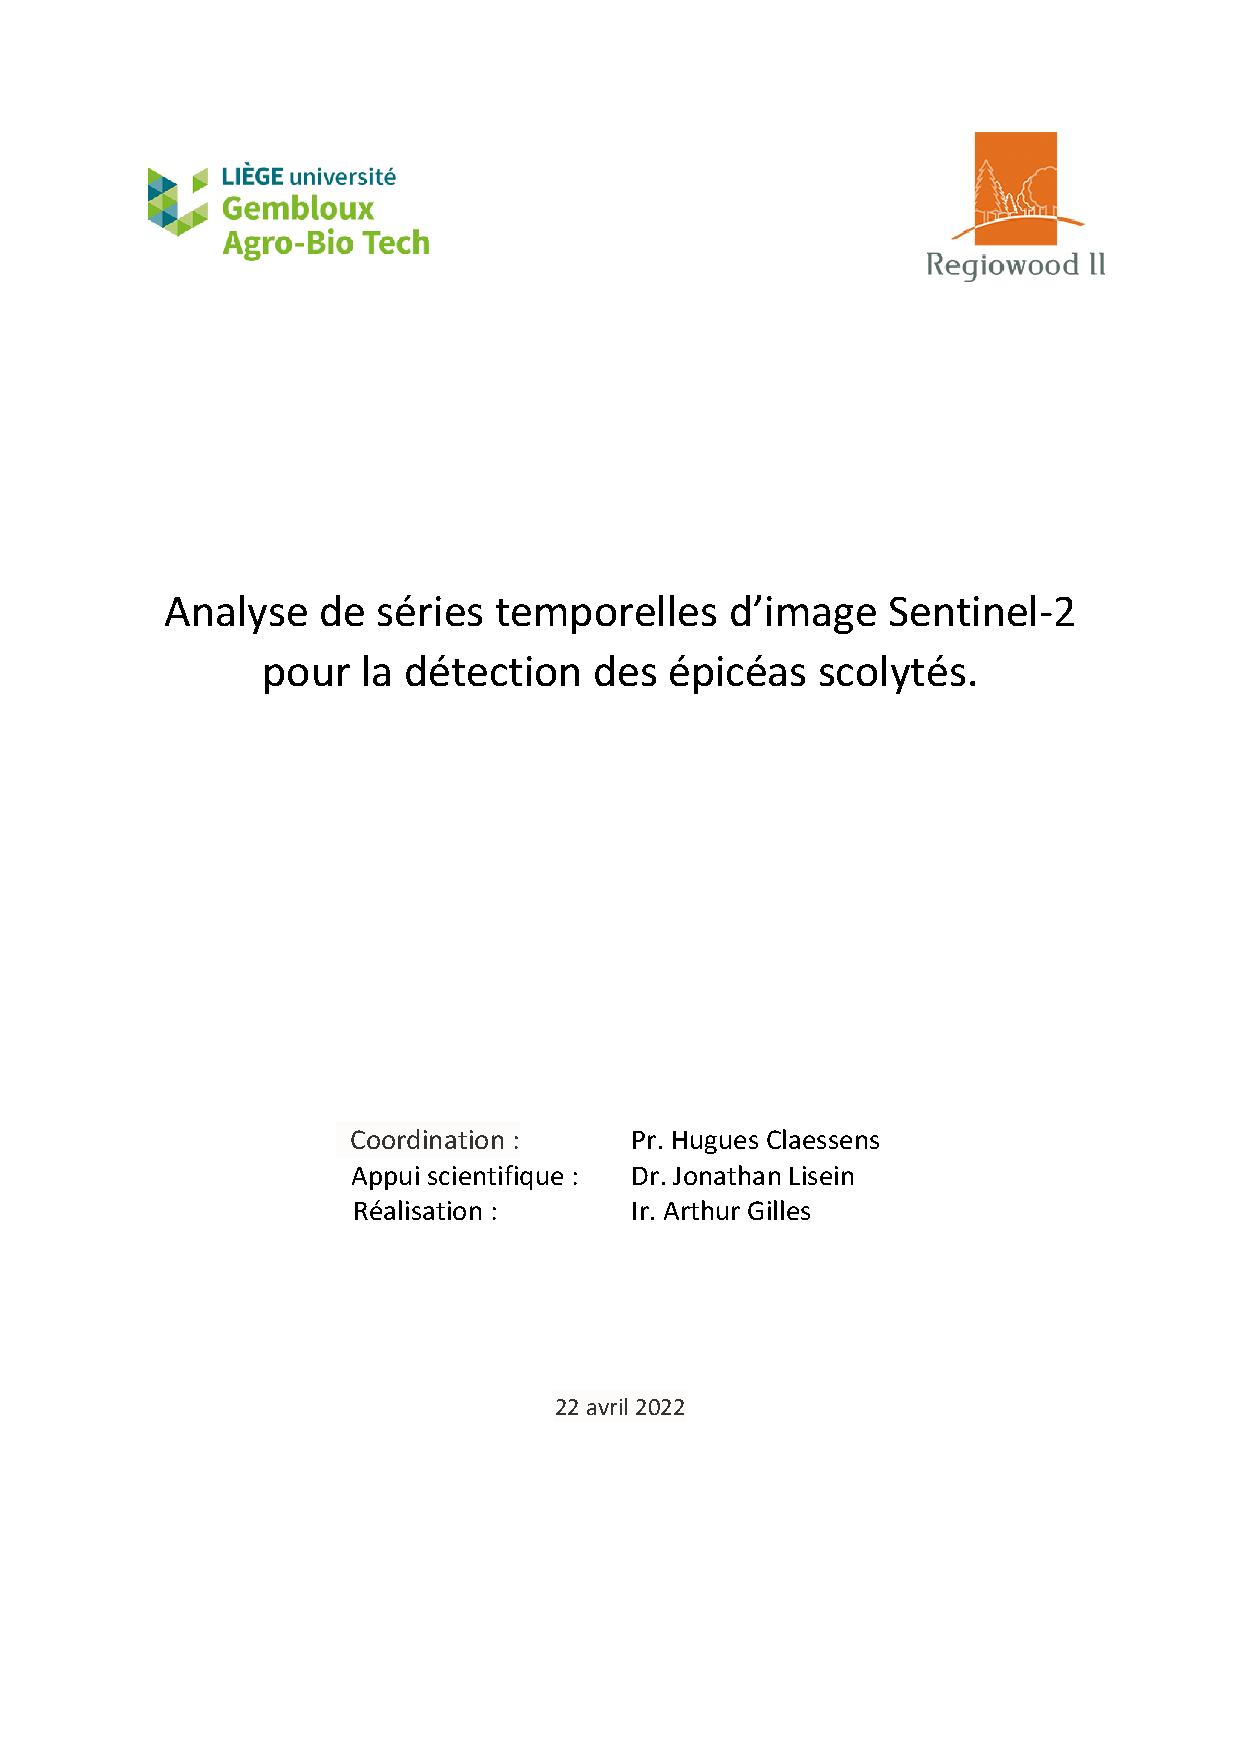
\includepdf[pages=-]{pages_Degarde_methodoAnalyseSentinel2.pdf} % page de titre fait dans word, plus maniable


\pagebreak
\tableofcontents
\pagebreak

\section{Introduction}

Dans le cadre du projet InterReg RegioWood 2 et de l'Accord cadre de recherche et vulgarisation forestière, la crise du typographe qui touche les pessières wallonnes est étudiée au moyen de la télédétection. L'objectif est de dresser des cartes d'état sanitaire pour chaque année étudiée sur lesquelles on puisse distinguer les arbres sains des arbres dépérissant. L'utilisation de série temporelle d'images satellites dispose d'un potentiel très intéressant pour le suivi de la phénologie des arbres.

%Le présent document est un document interne de l'unité de Gestion des ressources forestières (Ulg). Pour toutes questions ou remarques, contactez Lisein Jonathan par courriel (\href{mailto:liseinjon@hotmail.com}{liseinjon@hotmail.com}).

\subsection{Sentinel-2}

L'imagerie multispectrale des deux satellites Sentinel-2 (A et B, mis en orbite en juin 2015 et mars 2017) du programme Copernicus est à la base de la méthodologie présenté dans ce document. La résolution des bandes spectrales de Sentinel-2 est de 10 mètres dans le meilleurs des cas (certaines fréquences utilisées pour le suivi sanitaire sont captées à 20 mètres). La fréquence de revisite à l'équateur est de 5 jours, mais on dispose en Belgique de l'ordre d'une 12aine de prises de vue par an pour lesquelles la couverture nuageuse est suffisamment faible. Les prises de vue font l'objet de traitement et sont redécoupées selon un carroyage de tuiles carrées de 100km de côté (figure \ref{fig:tuileRW}). %Le shapefile des tuiles et des centroïdes sont disponible sous \url{https://github.com/justinelliotmeyers/Sentinel-2-Shapefile-Index}.

\begin{figure}[H]
\centering
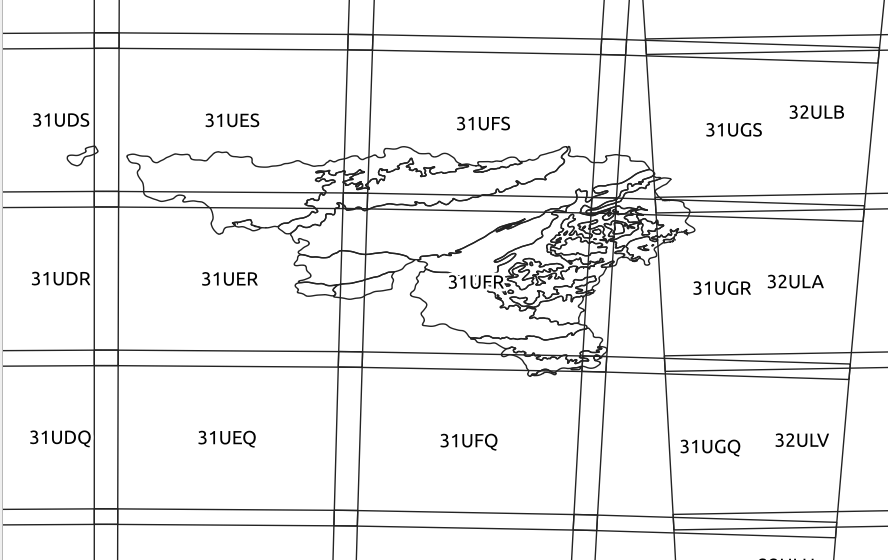
\includegraphics[width=0.9\linewidth]{../theia_d/tuileS2Nom.png}
\caption{La Wallonie est couverte par un total de 8 tuiles Sentinel-2, mais la tuile 31UFR couvre à elle seule une majorité de l'Ardenne Belge.}
\label{fig:tuileRW}
\end{figure}

\section{Méthodologie de la détection des typographes}

\subsection{Suivi d'un indice spectral pour la détection précoce de stress}\label{subsec:methodo}


L'idée générale est de se calquer sur la méthodologie de l'INRAE (INRAE, UMR TETIS, R. Dutrieux, K. Ose, J.-B. Féret : voir \citep{dutrieux_package_2021,dutrieux_mise_2021}) développée depuis 2017. 

L'indice spectral permettant la détection précoce (stade vert du dépérissement) des dépérissements provoqués par l'attaque de typographes est le CRSWIR :

%\begin{equation*}
\begin{align*} 
\mathbold{SWIR_{CR} = \dfrac{SWIR1}{( NIRa + (\lambda_{SWIR1}-\lambda_{NIRa})* (\dfrac{SWIR2 - NIRa}{\lambda_{SWIR2}-\lambda_{NIRa}})}} 
\\ 
avec&\\ 
\lambda_{NIRa} &=865\\ 
\lambda_{SWIR1} &=1610\\ 
\lambda_{SWIR2} &=2190
%\end{equation*}
\end{align*} 

A noter que CR est l'acronyme de \textit{continuum removal}, technique qui consiste à maximiser le contraste spectral associé à des pics d’absorption, en normalisant la valeur de réflectance
par rapport à la valeur d’une ‘enveloppe convexe’ calculée à partir de bandes spectrales voisines \citep{dutrieux_mise_2021}.
Les valeurs d'un peuplements soumis à un stress physiologique voient leur CRSWIR augmenter de manière précoce.

\begin{equation}\label{eq:harmo}
 f(t) =   a_{1} + b_{1} \sin(\dfrac{2\pi}{T}t)+ b_{2} \cos(\dfrac{2\pi}{T}t)+ b_{3} \sin(\dfrac{2\pi}{T}2t)+ b_{4} \cos(\dfrac{2\pi}{T}2t)
\end{equation} 

L'équation \ref{eq:harmo} permet de modéliser les variations saisonnières de CRSWIR pour un peuplement d'épicéa sain. La constante T est égal à 365,25. Cette équation ajustée sur 300 pessières saines est illustrée pour 3 années sur la figure \ref{fig:harmo}. Pour un pixel donnée, l'étude de la série temporelle de valeurs de CRSWIR, correspondant donc à chaque date pour lesquelles une image Sentinel-2 peu ennuagée est disponible, permet de déterminer si le peuplement est soumis à un stress. Plusieurs situations existent en dehors de celle d'une pessière saine et de celle d'une pessière scolytée. En effet, il est également nécessaire de déterminer si le peuplement est coupé (détection de sol nu), ou si le peuplement présente un stress temporaire dû probablement à un déficit hydrique temporaire. Les pessières sur des sols à régime hydrique alternatif sont fortement représentatives de cette dernière situation, avec typiquement un déficit hydrique estival entraînant un stress passager qui se manifestera par une augmentation de CRSWIR, mais qui se différentie d'une attaque de scolyte par un retour à un état sanitaire normal (diminution du CRSWIR) peu de temps après.

\begin{figure}[H]
	\centering
	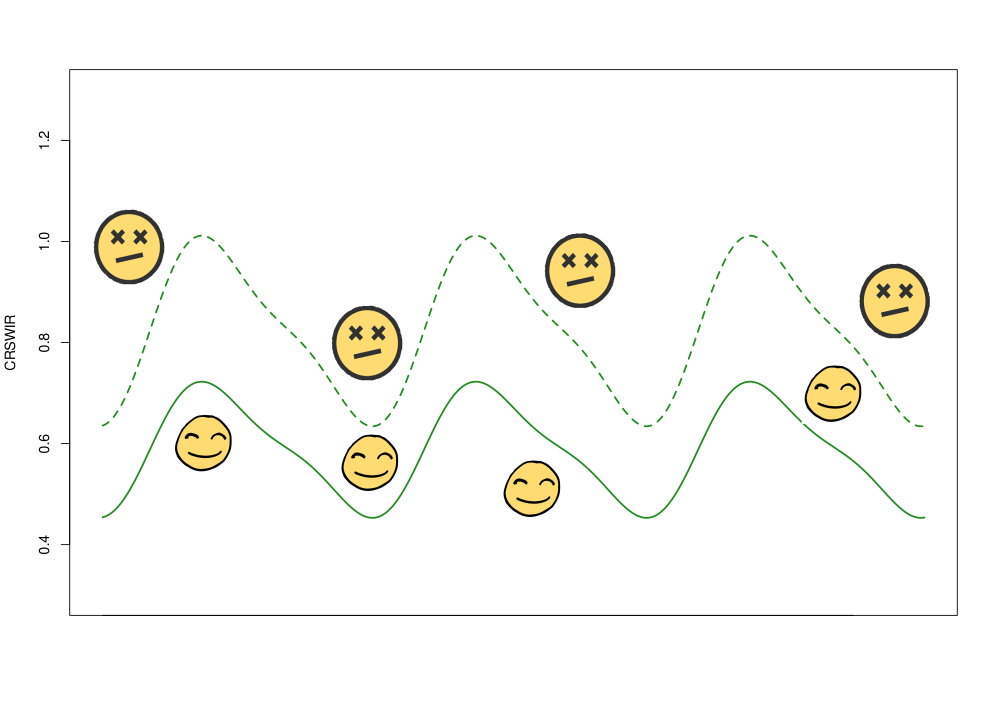
\includegraphics[width=0.9\linewidth]{fctHarmo.png}
	\caption{L'indice CRSWIR pour un peuplement sain varie durant l'année selon une fonction harmonique (trait plein en vert sur la figure). Un arbre dépérissant va présenter une valeur de CRSWIR qui sera supérieure à la normale. On décide arbitrairement que les valeurs qui dépassent la courbe en pointillé sont considérées comme représentative d'un stress. }
	\label{fig:harmo}
\end{figure}

Afin de faciliter la comparaison d'une valeur de CRSWIR pour une date donnée avec la valeur de référence, qui est la valeur de CRSWIR d'une pessière saine représenté par l'équation \ref{eq:harmo}, nous utilisons un ratio tel que défini ci-dessous :

\begin{equation}\label{eq:crswirnorm}
CR_{SWRIR_{norm}}(t)=\dfrac{CRSWIR_{observe}}{CRSWIR_{theorique}(t)}
\end{equation} 

le $CRSWIR_{theorique}(t)$ représente bien entendu la valeur calculée au moyen de l'équation \ref{eq:crswirnorm}. Le CRSWIR normalisé est donc un ratio qui, lorsque sa valeur est de 1, représente l'état typique d'une pessière saine, et lorsqu'il dépasse un certain seuil (fixé entre 1.5 et 1.7), est considéré comme représentatif d'un stress végétatif. Une fois le CRSWIR normalisé calculé pour chaque date de prise de vue, la suite des traitements peut s'effectuer sans à avoir à considérer la variation saisonnière inhérente au changements phénologiques de la végétation.

\begin{figure}[H]
	\centering
	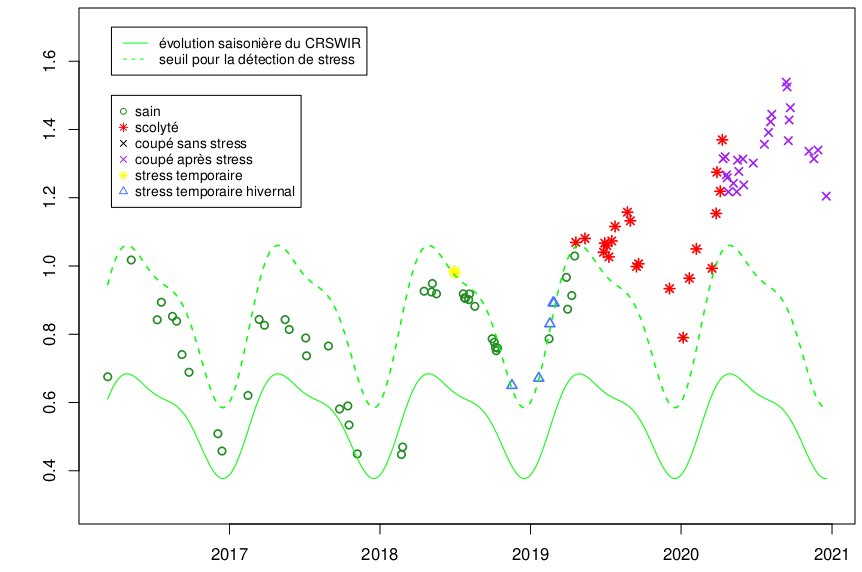
\includegraphics[width=0.9\linewidth]{illuArbreCoupe.png}
	\caption{Exemple d'une série temporelle d'observation de CRSWIR pour un pixel donné. Un état sanitaire présumé est attribué à chaque observation en fonction de la valeur de CRSWIR, de la présence ou non de sol nu et à son état sanitaire pour les dates antérieures et postérieures. Par exemple, en 2020, l'état sanitaire attribué est celui "coupé après stress" (croix mauve sur le graphique) car d'une part le pixel est détecté comme étant en sol nu, d'autre part les observations antérieures (été 2019 et hiver 2020) sont considérées comme étant "scolytées" (étoile rouge sur le graphique) }
	\label{fig:ex}
\end{figure}

\subsection{Ensemble de règles pour attribuer un état sanitaire}\label{subsec:ES}

\begin{enumerate}
	%code 1
	\item \crule[cl1]{1cm}{1cm} ; sain 
	%code 2
	\item \crule[cl2]{1cm}{1cm} ; dépérissement 
	%code 3
	\item \crule[cl3]{1cm}{1cm} ; coupé mais sans dépérissement détecté avant la coupe 
	%code 4
	\item  \crule[cl4]{1cm}{1cm} ;coupé après avoir été dépérissant
	%code 5
	\item \crule[cl5]{1cm}{1cm} ; stress passager, donc à priori plus un stress lié à un déficit hydrique estival qu'à une attaque de scolyte. 
	%code 6
	\item \crule[cl6]{1cm}{1cm} ; pixel qui est un mélange, détecté car présente un stress passager en hiver (feuillus sans photosynthèse) suivi d'un retour à la normale en été (résineux + feuillus en photosynthèse) 
\end{enumerate}

Les filtres et les règles de décisions permettant d'attribuer un état sanitaire à une observation d'une série temporelle sont brièvement présentés dans cette partie. On peut considérer que la série temporelle pour un pixel donné est synthétisée sous forme d'un tableau à 2 colonnes pour lequel chaque ligne constitue une date pour laquelle on dispose d'une information (prise de vue non ennuagée pour cette position). La première colonne est celle contenant l'information de la date de l'observation. La deuxième colonne contient un état sanitaire présumé, qui peut prendre la valeur de 1, 2 ou 3 avant de subir l'analyse présentée ici. La valeur de 1 signifie que la valeur de CRSWIR permet de supposer que le peuplement est sain. La valeur de 2 indique par contre que le peuplement semble en situation de stress, avec un $CRSWIR_{normalise}$ supérieur au seuil fixé (ex. 1.4, voir ligne en pointillé de la figure \ref{fig:harmo}).

L'analyse commence par un premier filtre qui vise à retirer les valeurs aberrantes de la série temporelle. On va pour ce faire contrôler que aucune valeur de 2 (stress) ou 3 (coupé) n'apparaît de manière isolée. L'hypothèse est simplement qu'un pixel détecté comme stressé à une date mais considéré comme sain à la date précédente à la date suivante correspond à une observation aberrante qui sera donc retiré ici.

Ensuite, un deuxième filtre vise à classer les coupes (code 3) et les coupes sanitaires (code 4). On va pour se faire identifier toutes les occurrences d'au moins 3 détection de sol nu consécutifs, ou encore de 2 détections de sol nu mais dont les 2 dates sont séparées d'au moins 40 jours (pour considérer les situations de sols nus au dessus d'une zone fortement ennuagé et donc avec une densité temporelle d'observations assez faible). Lorsqu'une situation similaire est détectée, l'état de toutes les observations suivantes sont fixées à "coupé" ou à "coupe sanitaire" si un stress a été détecté à la date antérieure à la détection du sol nu. L'idée est bien d'éviter qu'une position détectée comme sol nu ne soit classée comme étant une pessière saine les mois et années suivant la coupe. Nous attirons l'attention que la méthodologie employée ici sur des images de 10m de résolution n'a pas pour objectif d'obtenir de bons résultats sur des jeunes plantations, pour lesquels la réponse spectrale est un mélange résultant de celle des petits houppiers et de la végétation environnante.

La troisième partie de l'analyse vise à la détection des situations de peuplements scolytés. Si un stress est observé plusieurs fois d'affilé, on va modifier les états sanitaires postérieurs pour s'assurer que ceux-ci correspondent soit à un stress, soit à une coupe sanitaire. Néanmoins, un \textit{retour à une situation normale} est accepté dans le cas ou un état sanitaire sain est constaté plus de 3 fois consécutivement, pour une durée excédant 30 jours et seulement dans les cas ou le dépérissement observé précédemment n'as pas duré plus longtemps qu'un certain nombre de jours (par défaut 90 jours mais augmenté à 150 jours pour la version 2022 des cartes d'état sanitaire). Lorsqu'un \textbf{retour à la normale} est ainsi détecté, l'état sanitaire durant la période de stress est considéré comme étant un stress temporaire (code 5) et non pas une situation de présence de scolyte.

Enfin, un dernier filtre permet d'appréhender la situation assez complexe mais marginale d'un pixel qui couvrirait une surface hétérogène du point de vue de la présence de l'épicéa, tels qu'un mélange épicéa-feuillus ou un mélange épicéa-sol nu. La détection de mélange vise à réduire le taux de faux positif pour les zones scolytés.

\subsection{Illustrations des cartes d'état sanitaire}

Les illustrations suivantes montrent à quoi ressemble les cartes d'état sanitaire sur de petites zones, celles-ci étant accompagnés des prises de vues aériennes de la Région wallonne afin de donner un visuel du peuplement.

\begin{figure}
	\begin{minipage}[b]{.32\linewidth}
		\centering ortho 2018
		\subcaption{\includegraphics[width=\linewidth]{etatSan/1/ortho_2018.png_LR.png}}
	\end{minipage}%
	\begin{minipage}[b]{.32\linewidth}
		\centering IR 2018
		\subcaption{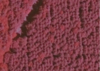
\includegraphics[width=\linewidth]{etatSan/1/IR_2018.png_LR.png}}
	\end{minipage}
	\begin{minipage}[b]{.32\linewidth}
	\centering état sanitaire 2018
	\subcaption{
\includegraphics[width=\linewidth]{etatSan/1/ES_2018.png_LR.png}}
\end{minipage}
\begin{minipage}[b]{.32\linewidth}
	\centering ortho 2019
	\subcaption{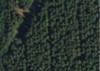
\includegraphics[width=\linewidth]{etatSan/1/ortho_2019.png_LR.png}}
\end{minipage}%
\begin{minipage}[b]{.32\linewidth}
	\centering IR 2019
	\subcaption{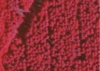
\includegraphics[width=\linewidth]{etatSan/1/IR_2019.png_LR.png}}
\end{minipage}
\begin{minipage}[b]{.32\linewidth}
	\centering état sanitaire 2019
	\subcaption{
\includegraphics[width=\linewidth]{etatSan/1/ES_2019.png_LR.png}}
\end{minipage}
\begin{minipage}[b]{.32\linewidth}
	\centering ortho 2020
	\subcaption{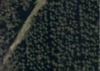
\includegraphics[width=\linewidth]{etatSan/1/ortho_2020.png_LR.png}}
\end{minipage}
\begin{minipage}[b]{.32\linewidth}
	\centering IR 2020
	\subcaption{\includegraphics[width=\linewidth]{etatSan/1/IR_2020.png_LR.png}}
\end{minipage}
\begin{minipage}[b]{.32\linewidth}
	\centering état sanitaire 2020
	\subcaption{
\includegraphics[width=\linewidth]{etatSan/1/ES_2020.png_LR.png}}
\end{minipage}
	\caption{Illustration pour une pessière saine \crule[cl1]{1cm}{1cm}}\label{fig:illuCl1}
\end{figure}


\begin{figure}
	\begin{minipage}[b]{.32\linewidth}
		\centering ortho 2018
		\subcaption{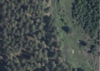
\includegraphics[width=\linewidth]{etatSan/2/ortho_2018.png_LR.png}}
	\end{minipage}%
	\begin{minipage}[b]{.32\linewidth}
		\centering IR 2018
		\subcaption{\includegraphics[width=\linewidth]{etatSan/2/IR_2018.png_LR.png}}
	\end{minipage}
	\begin{minipage}[b]{.32\linewidth}
		\centering état sanitaire 2018
		\subcaption{
\includegraphics[width=\linewidth]{etatSan/2/ES_2018.png_LR.png}}
	\end{minipage}
	\begin{minipage}[b]{.32\linewidth}
		\centering ortho 2019
		\subcaption{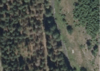
\includegraphics[width=\linewidth]{etatSan/2/ortho_2019.png_LR.png}}
	\end{minipage}%
	\begin{minipage}[b]{.32\linewidth}
		\centering IR 2019
		\subcaption{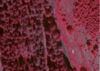
\includegraphics[width=\linewidth]{etatSan/2/IR_2019.png_LR.png}}
	\end{minipage}
	\begin{minipage}[b]{.32\linewidth}
		\centering état sanitaire 2019
		\subcaption{
\includegraphics[width=\linewidth]{etatSan/2/ES_2019.png_LR.png}}
	\end{minipage}
	\begin{minipage}[b]{.32\linewidth}
		\centering ortho 2020
		\subcaption{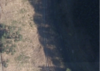
\includegraphics[width=\linewidth]{etatSan/2/ortho_2020.png_LR.png}}
	\end{minipage}
	\begin{minipage}[b]{.32\linewidth}
		\centering IR 2020
		\subcaption{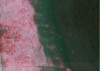
\includegraphics[width=\linewidth]{etatSan/2/IR_2020.png_LR.png}}
	\end{minipage}
	\begin{minipage}[b]{.32\linewidth}
		\centering état sanitaire 2020
		\subcaption{
\includegraphics[width=\linewidth]{etatSan/2/ES_2020.png_LR.png}}
	\end{minipage}
	\caption{Illustration pour une pessière scolytée \crule[cl2]{1cm}{1cm} }\label{fig:illuCl2}
\end{figure}

\begin{figure}
	\begin{minipage}[b]{.32\linewidth}
		\centering ortho 2018
		\subcaption{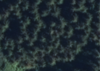
\includegraphics[width=\linewidth]{etatSan/3/ortho_2018.png_LR.png}}
	\end{minipage}%
	\begin{minipage}[b]{.32\linewidth}
		\centering IR 2018
		\subcaption{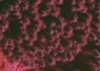
\includegraphics[width=\linewidth]{etatSan/3/IR_2018.png_LR.png}}
	\end{minipage}
	\begin{minipage}[b]{.32\linewidth}
		\centering état sanitaire 2018
		\subcaption{
\includegraphics[width=\linewidth]{etatSan/3/ES_2018.png_LR.png}}
	\end{minipage}
	\begin{minipage}[b]{.32\linewidth}
		\centering ortho 2019
		\subcaption{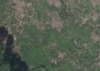
\includegraphics[width=\linewidth]{etatSan/3/ortho_2019.png_LR.png}}
	\end{minipage}%
	\begin{minipage}[b]{.32\linewidth}
		\centering IR 2019
		\subcaption{\includegraphics[width=\linewidth]{etatSan/3/IR_2019.png_LR.png}}
	\end{minipage}
	\begin{minipage}[b]{.32\linewidth}
		\centering état sanitaire 2019
		\subcaption{
\includegraphics[width=\linewidth]{etatSan/3/ES_2019.png_LR.png}}
	\end{minipage}
		
	\begin{minipage}[b]{.32\linewidth}
		\centering ortho 2020
		\subcaption{\includegraphics[width=\linewidth]{etatSan/3/ortho_2020.png_LR.png}}
	\end{minipage}
	\begin{minipage}[b]{.32\linewidth}
		\centering IR 2020
		\subcaption{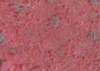
\includegraphics[width=\linewidth]{etatSan/3/IR_2020.png_LR.png}}
	\end{minipage}
	\begin{minipage}[b]{.32\linewidth}
		\centering état sanitaire 2020
		\subcaption{
\includegraphics[width=\linewidth]{etatSan/3/ES_2020.png_LR.png}}
	\end{minipage}
	\caption{Illustration pour une pessière détectée en coupe \crule[cl3]{1cm}{1cm}}\label{fig:illuCl3}
\end{figure}

\begin{figure}
	\begin{minipage}[b]{.32\linewidth}
		\centering ortho 2018
		\subcaption{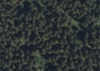
\includegraphics[width=\linewidth]{etatSan/4/ortho_2018.png_LR.png}}
	\end{minipage}%
	\begin{minipage}[b]{.32\linewidth}
		\centering IR 2018
		\subcaption{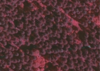
\includegraphics[width=\linewidth]{etatSan/4/IR_2018.png_LR.png}}
	\end{minipage}
	\begin{minipage}[b]{.32\linewidth}
		\centering état sanitaire 2018
		\subcaption{
\includegraphics[width=\linewidth]{etatSan/4/ES_2018.png_LR.png}}
	\end{minipage}
	\begin{minipage}[b]{.32\linewidth}
		\centering ortho 2019
		\subcaption{\includegraphics[width=\linewidth]{etatSan/4/ortho_2019.png_LR.png}}
	\end{minipage}%
	\begin{minipage}[b]{.32\linewidth}
		\centering IR 2019
		\subcaption{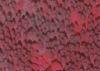
\includegraphics[width=\linewidth]{etatSan/4/IR_2019.png_LR.png}}
	\end{minipage}
	\begin{minipage}[b]{.32\linewidth}
		\centering état sanitaire 2019
		\subcaption{
\includegraphics[width=\linewidth]{etatSan/4/ES_2019.png_LR.png}}
	\end{minipage}
	
	\begin{minipage}[b]{.32\linewidth}
		\centering ortho 2020
		\subcaption{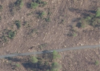
\includegraphics[width=\linewidth]{etatSan/4/ortho_2020.png_LR.png}}
	\end{minipage}
	\begin{minipage}[b]{.32\linewidth}
		\centering IR 2020
		\subcaption{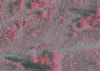
\includegraphics[width=\linewidth]{etatSan/4/IR_2020.png_LR.png}}
	\end{minipage}
	\begin{minipage}[b]{.32\linewidth}
		\centering état sanitaire 2020
		\subcaption{
\includegraphics[width=\linewidth]{etatSan/4/ES_2020.png_LR.png}}
	\end{minipage}
	\caption{Illustration pour une pessière détectée en coupe sanitaire \crule[cl4]{1cm}{1cm}}\label{fig:illuCl4}
\end{figure}

\iffalse

\begin{figure}
	\begin{minipage}[b]{.32\linewidth}
		\centering ortho 2018
		\subcaption{\includegraphics[width=\linewidth]{etatSan/5/ortho_2018.png_LR.png}}
	\end{minipage}%
	\begin{minipage}[b]{.32\linewidth}
		\centering IR 2018
		\subcaption{\includegraphics[width=\linewidth]{etatSan/5/IR_2018.png_LR.png}}
	\end{minipage}
	\begin{minipage}[b]{.32\linewidth}
		\centering état sanitaire 2018
		\subcaption{
\includegraphics[width=\linewidth]{etatSan/5/ES_2018.png_LR.png}}
	\end{minipage}
	\begin{minipage}[b]{.32\linewidth}
		\centering ortho 2019
		\subcaption{\includegraphics[width=\linewidth]{etatSan/5/ortho_2019.png_LR.png}}
	\end{minipage}%
	\begin{minipage}[b]{.32\linewidth}
		\centering IR 2019
		\subcaption{\includegraphics[width=\linewidth]{etatSan/5/IR_2019.png_LR.png}}
	\end{minipage}
	\begin{minipage}[b]{.32\linewidth}
		\centering état sanitaire 2019
		\subcaption{
\includegraphics[width=\linewidth]{etatSan/5/ES_2019.png_LR.png}}
	\end{minipage}
	\begin{minipage}[b]{.32\linewidth}
		\centering ortho 2020
		\subcaption{\includegraphics[width=\linewidth]{etatSan/5/ortho_2020.png_LR.png}}
	\end{minipage}
	\begin{minipage}[b]{.32\linewidth}
		\centering IR 2020
		\subcaption{\includegraphics[width=\linewidth]{etatSan/5/IR_2020.png_LR.png}}
	\end{minipage}
	\begin{minipage}[b]{.32\linewidth}
		\centering état sanitaire 2020
		\subcaption{
\includegraphics[width=\linewidth]{etatSan/5/ES_2020.png_LR.png}}
	\end{minipage}
	\caption{Illustration pour une pessière soumis à un stress temporaire \crule[cl5]{1cm}{1cm} }\label{fig:illuCl5}
\end{figure}


\begin{figure}
	\begin{minipage}[b]{.32\linewidth}
		\centering ortho 2018
		\subcaption{\includegraphics[width=\linewidth]{etatSan/6/ortho_2018.png_LR.png}}
	\end{minipage}%
	\begin{minipage}[b]{.32\linewidth}
		\centering IR 2018
		\subcaption{\includegraphics[width=\linewidth]{etatSan/6/IR_2018.png_LR.png}}
	\end{minipage}
	\begin{minipage}[b]{.32\linewidth}
		\centering état sanitaire 2018
		\subcaption{\includegraphics[width=\linewidth]{etatSan/6/ES_2018.png_LR.png}}
	\end{minipage}
	\begin{minipage}[b]{.32\linewidth}
		\centering ortho 2019
		\subcaption{\includegraphics[width=\linewidth]{etatSan/6/ortho_2019.png_LR.png}}
	\end{minipage}%
	\begin{minipage}[b]{.32\linewidth}
		\centering IR 2019
		\subcaption{\includegraphics[width=\linewidth]{etatSan/6/IR_2019.png_LR.png}}
	\end{minipage}
	\begin{minipage}[b]{.32\linewidth}
		\centering état sanitaire 2019
		\subcaption{\includegraphics[width=\linewidth]{etatSan/6/ES_2019.png_LR.png}}
	\end{minipage}
	
	\begin{minipage}[b]{.32\linewidth}
		\centering ortho 2020
		\subcaption{\includegraphics[width=\linewidth]{etatSan/6/ortho_2020.png_LR.png}}
	\end{minipage}
	\begin{minipage}[b]{.32\linewidth}
		\centering IR 2020
		\subcaption{\includegraphics[width=\linewidth]{etatSan/6/IR_2020.png_LR.png}}
	\end{minipage}
	\begin{minipage}[b]{.32\linewidth}
		\centering état sanitaire 2020
		\subcaption{\includegraphics[width=\linewidth]{etatSan/6/ES_2020.png_LR.png}}
	\end{minipage}
	\caption{Illustration pour des pixels détectés comme étant en mélange \crule[cl6]{1cm}{1cm}}\label{fig:illuCl6}
\end{figure}

\fi
\subsection{Délais de coupe et première date de détection de scolyte}

Les résultats de la détection des scolytes par analyse de série temporelle sont résumés sous forme de carte d'état sanitaire annuelle. Disposer d'un état sanitaire par année est un compromis de synthèse, afin de simplifier l'information tout en disposant de suffisamment de détails. Néanmoins, il peut s'avérer nécessaire d'utiliser d'autres informations, tels que, pour un peuplement en éclaircie sanitaire, le délais de coupe. Egalement, la première date de détection d'une attaque de scolyte est aussi intéressante, d'une part pour un suivi plus fin des foyers de scolyte, d'autre part pour la validation de la carte d'état sanitaire par photointerprétation des orthophotomosaiques annuelles de la Région wallonne.
Les cartes de délais de coupe et de première apparition des scolytes peuvent être exportées de manière optionnelle. Il s'agit, comme pour les cartes d'état sanitaire, d'une série temporelle de carte à raison de une par année.
L'information ne sera pertinente que pour la première année d'attaque de scolyte. 
Si un peuplement est attaqué en 2017, la carte de délais de coupe et de première date d'attaque pour l'année  2018 contiendra une valeur nulle.
Ces cartes sont de format 8bits, avec des valeurs comprises entre 0 et 255.
Afin d'éviter un dépassement de valeurs de nombre de jours qui peuvent en théorie atteindre le maximum de 365 jours (une année), le délais de coupe et la date de première attaque sont exprimées en nombre de semaines. Pour la date de première attaque, il s'agit du nombre de semaine depuis le début de l'année en cours, additionné de 100. Attention, les années sont des périodes de végétation qui commence en mai pour terminer en avril de l'année civile suivantes.

%Par ailleurs, la valeur spéciale 255 signifie que le pixel a été attaqué et/ou coupé l'année précédente. La valeur de 0, elle, est utilisée si le pixel n'est pas dans le masque forestier ou si aucune attaque de scolyte n'est à constater.

\iffalse
\section{Le logiciel s2{\textunderscore}timeSerie}

Bien que conceptuellement la méthode ne soit pas extrêmement compliquée, le volume de donnée est considérable et nécessite une organisation soigneuse ainsi qu'une méthode de calcul optimisée. C'est dans ce but qu'est développé l'application \textbf{s2{\textunderscore}timeSerie}, sous C++ et dans un environnement Linux.

L'application a été développée au départ avec une série d'arguments optionnels que l'utilisateur renseignait lors du lancement de l'application, de la manière suivante :

%--dates 2016-01-01 2017-01-01 
\begin{lstlisting}
./s2_timeSerie --catalogue 1 --tuile T32ULU 
./s2_timeSerie --catalogue 2 --tuile T31UGR --srCR 1.7
\end{lstlisting}

l'argument \textbf{tuile} renseigne le nom de une ou plusieurs tuiles Sentinel-2.
l'argument \textbf{catalogue} peut recevoir les valeurs de 1 ou de 2. Deux modes de création d'un catalogue, c'est à dire d'une série temporelle d'images pour une tuile donnée, sont disponibles.

Avec le mode 1, \textbf{s2{\textunderscore}timeSerie} effectue le téléchargement des données depuis la plateforme theia. Les informations nécessaires sont le nom de la tuile Sentinel-2 et une plage de date durant laquelle on souhaite effectuer l'analyse. Cette plage de date peux être définie avec l'argument --dates . par exemple : --dates 2016-01-01 2017-01-01.

Avec le mode 2 (--catalogue 2), le catalogue est créé sur base des dossiers téléchargés précédemment. Chaque dossier correspond à une date de prise de vue. Seul le nom de la tuile est donc requis.

La complexité grandissantes du jeu de donnée nous a obligé à changer la manière dont les paramètres sont renseignés. 
Maintenant, les paramètres sont renseignés au moyen d'un fichier xml qui présente une structure telle que celle-ci:
\lstset{language=XML}
\begin{lstlisting}
<params>

<path_otb>/home/gef/Documents/OTB-7.2.0-Linux64/bin/</path_otb>
<EP_mask_path>/home/gef/Documents/input/masque_EP.tif</EP_mask_path>
<suffix></suffix>
<catalogueMode> 2 </catalogueMode> <!-- 1 ; téléchargement. 
2 : pas de téléchargement -->
<doAnaTS> 1 </doAnaTS>
<debugDetail>0</debugDetail>

<doDelaisCoupe>1</doDelaisCoupe>
<doFirstDateSco>1</doFirstDateSco>

<Tuiles>
	<Tuile name="T31UER">
		<wd>/media/gef/Data2/S2Scolyte/</wd>
		<doTuile>0</doTuile>
	</Tuile>
	<Tuile name="T31UES">
		<wd>/media/gef/Data2/S2Scolyte/</wd>
		<doTuile>0</doTuile>
	</Tuile>
	<Tuile name="T31UFQ">
		<wd>/media/gef/Data2/S2Scolyte/</wd>
		<doTuile>0</doTuile>
	</Tuile>
	<Tuile name="T31UFR">
		<wd>/media/gef/Data2/S2Scolyte/</wd>
		<doTuile>0</doTuile>
	</Tuile>
	<Tuile name="T31UFS">
		<wd>/media/gef/Data2/S2Scolyte/</wd>
		<doTuile>0</doTuile>
	</Tuile>
	<Tuile name="T31UGR">
		<wd>/media/gef/Data2/S2Scolyte/</wd>
		<doTuile>0</doTuile>
	</Tuile>
	<Tuile name="T31UGS">
		<wd>/media/gef/Datas/S2Scolyte/</wd>
		<doTuile>1</doTuile>
	</Tuile>
</Tuiles>
</params>
\end{lstlisting}

Ce sytème offre plus de flexibilité, à savoir
\begin{itemize}
	\item renseigner une liste de tuiles et leur chemin d'accès. Les séries temporelles de deux tuiles différentes ne doivent pas nécessairement être sur le même disque dur.
	\item renseigner un masque global (=qui couvre plusieurs tuiles, ex masque épicéa en RW) ainsi qu'un suffix qui sera utilisé pour tout les résultats intermédiaire et finaux. Cela permet d'effectuer l'analyse sur des zones différentes, ce qui n'était pas prévu initialement.
	\item un fichier xml offre une manipulation plus aisée dès qu'il s'agit de renseigner un nombre très élevés de paramètres.
\end{itemize}

Le fichier xml est passé en argument lors de l'appel à l'outil \textbf{s2{\textunderscore}timeSerie}:
\begin{lstlisting}
./s2_timeSerie --xmlIn ./s2_scoBelgique.xml 
\end{lstlisting}

L'appli utilise OTB comme calculatrice raster, pour tout ce qui concerne les éléments ci-dessous :
\begin{itemize}
	\item calcul de cartes de masques (no data et nuage)
	\item rééchantillonnage des bandes spectrales de Sentinel-2 de 20m vers 10m de résolution
	\item calcul de carte pour la détection du sol nu
	\item le calcul des cartes de CRSWIR
	\item le calcul des cartes de CRSWIR normalisé
\end{itemize}

L'ensemble de ces opérations sont effectuées date par date de manière indépendante, et restent donc de l'ordre du monotemporel. Leur relative simplicité font que ces opérations sont considérées comme des prétraitements. Ces prétraitements sont évidemment préliminaires à l'analyse de la série temporelle à proprement parler.
 
\subsection{Organisation du code source}

Trois classes d'objets sont définies dans le projet C++ et permettent d'effectuer toutes les opérations nécessaires. Ces classes sont présentées brièvement ci-dessous. Ces informations sont une aide destinée à l'utilisateur qui souhaite lire le code source pour le comprendre et/ou le modifier. La figure \ref{fig:classes} schématise le fonctionnement des 3 classes d'objets les unes par rapports aux autres.

\begin{figure}
	\centering
	\includegraphics[width=\linewidth]{illuAppliS2TS.png}
	\caption{L'application est développé avec l'approche de programmation Orientée Objet, dont les 3 classes principales sont les classes \textbf{catalogue}, \textbf{tuileS2OneDate} et \textbf{TS1Pos} représenté sur ce graphique.\textbf{}}
	\label{fig:classes}
\end{figure}

Afin de pouvoir utiliser ces classes dans différentes applications, des classes de bases sont développées pour \textbf{catalogue} et \textbf{tuileS2OneDate}. Des classes plus spécialisées héritent ensuite de ces trois classes de bases en fonction des objectifs poursuivis. Ainsi, pour la détection des scolytes, les classes \textbf{catalogueSco} et \textbf{tuileS2OneDateSco}  sont spécialisées.


\subsection{La classe \textbf{catalogue}}

C'est la classe qui contient toute la série temporelle sur l'emprise d'une tuile. La série temporelle est consituée par l'ensemble des prises de vue sur cette tuile. Les prises de vue retenues sont celles qui présentent un taux d'ennuagement inférieur à un seuil fixé à 35\%. C'est au niveau de cette classe que sont défini les dates de début et de fin de la série temporelle, mais aussi que la zone d'intérêt pour laquelle on souhaite effectuer les calculs est définie. En effet, l'analyse n'est pas effectuée sur l'ensemble du territoire mais uniquement sur les zones considérées comme étant des pessières. Le masque épicéa est donc utilisé comme donnée d'entrée et ce masque, qui couvre toute la Wallonie, est découpée par la classe catalogue afin d'épouser l'emprise de la tuile.

\subsection{La classe \textbf{tuileS2OneDate}}
C'est la classe qui contient toutes les informations relatives à une tuile pour une date donnée ; archive compressée, décompressée, métadonnées (date, nuage, nom du produit, répertoire ou j'ai mis les images, ect). Cette classe effectue la lecture de nombreuses informations depuis le fichier XML de métadonnées du produit Sentinel-2A pour cette date. Plus d'informations sont disponibles sous le lien \url{https://labo.obs-mip.fr/multitemp/sentinel-2/theias-sentinel-2-l2a-product-format/} à propos du format de données des produits 2A de Sentinel-2.

Les objets \textbf{tuileS2OneDate} regroupent l'ensemble des images nécessaires à l'analyse temporelle pour la détection de stress provoqué par les scolytes. En plus des images de chaque bande spectrale du capteur de Sentinel-2, les images calculés par OTB listées précédemment dans ce document sont gérées par la classe \textbf{tuileS2OneDate}.

\subsection{La classe \textbf{TS1Pos}}
C'est la classe qui effectue l'analyse de la série temporelle (\textbf{TS} pour Time Serie) pour une position donnée (\textbf{Pos} pour Position, qui est représenté par le centre de chaque pixels de l'image). C'est avec cette classe que l'on fait l'analyse de la succession de l'état sanitaire pour déterminer si la pessière en ce point est scolytée, coupée, saine, etc. La classe \textbf{TS1Pos} n'effectue aucune opération cartographique, c'est strictement l'analyse du CRSWIR normalisé au fil du temps, combiné avec la détection ou non de sol nu, qui sert d'information. Outre l'analyse de la série temporelle pour une position, cette classe a une méthode pour exporter un résultat synthétique pour cette position, en l'occurence un état sanitaire \textit{synthétique} pour chaque année. En effet, disposer d'un état sanitaire pour chaque année est un compromis entre trop de détails et trop de synthèse.

\fi

%\section{Les post-traitements avec s2{\textunderscore}postProcess}

\subsection{Les post-traitements}

Les traitements illustrés jusqu'à présent sont des calculs qui s'effectuent sur base de la série temporelle, mais sans prendre en compte les effets de voisinage. On peut dire que la dimension spatiale n'est pas prise en compte. Pour assurer une certaine cohérence dans les classes d'état sanitaire assignées à chaque pixel dans les cartes annuelles, un certain nombre de post traitement sont effectués et développés dans une seconde application. Cette application est assez polyvalente, avec un nombre d'outils assez élevés. Les outils permettent les actions suivantes ;
\begin{enumerate}\addtocounter{enumi}{-1}
	
	\item masquer les cartes d'états sanitaires avec la carte de pourcentage de GHA de l'épicéa (travaux de \citep{bolyn_forest_2018}), en utilisant un seuil de présence spécifié. Pour rappel, l'analyse de la série temporelle est effectué sur une zone définie sur base d'un pourcentage de GHA de l'épicéa de plus de 50\%. On peut donc avec cet outil se montrer plus restrictif en augmentant ce seuil, par exemple avec un seuil de 80\%.
	\item nettoyage des cartes d'état sanitaire. Pour le moment, il s'agit uniquement de localiser les zones de coupe non-sanitaire de petites dimensions qui sont entourées d'une coupe sanitaire. On met l'hypothèse que ces épicéas ont également été attaqués par le scolyte avant d'être abattu, comme leurs voisins directs, et on change la classe pour les mettre en coupe sanitaire.
	\item calcul des cartes d'évolutions de l'état sanitaire. Chaque carte d'état sanitaire est comparée avec celle de l'année précédente afin de classer les zones de scolyte en nouveau scolyte ou ancien scolyte, et les zones de coupe sanitaire en nouvelle ou ancienne coupe sanitaire. On distingue les nouvelles coupes sanitaires pour les peuplements scolytés durant l'année en cours des nouvelles coupes sanitaires pour les peuplement qui étaient déjà scolyté l'année précédente.
	\item  compression des cartes geotiff
	\item calcul de statistique (surface) pour chaque classe d'état sanitaire.
	\item projection des cartes vers le SRC 31370 Belge Lambert 72.
%	\item Extraction de valeurs d'état sanitaire pour les points d'un shapefile, dans un objectif de validation de la méthodo. Diverses indices de voisinage sont également calculé, comme la distance la plus proche à un foyer de scolyte.
\end{enumerate}

Voici les codes pour l'évolution de l'état sanitaire ainsi que la couleur associée:
\begin{enumerate}\setcounter{enumi}{20}
	\item \crule[cl21]{1cm}{1cm} ; ancien scolyte
	\item \crule[cl22]{1cm}{1cm} ; nouveau scolyte
	\setcounter{enumi}{40}
	\item \crule[cl41]{1cm}{1cm} ; ancienne coupe sanitaire
	\item \crule[cl42]{1cm}{1cm} ; nouvelle coupe sanitaire nouveau scolyte
	\item \crule[cl43]{1cm}{1cm} ; nouvelle coupe sanitaire ancien scolyte
\end{enumerate} 


\begin{figure}
\begin{minipage}[b]{.49\linewidth}
	\centering état sanitaire
	\subcaption{\includegraphics[width=\linewidth]{esAvantClean.png}}
\end{minipage}%
\begin{minipage}[b]{.49\linewidth}
	\centering état sanitaire après nettoyage
	\subcaption{\includegraphics[width=\linewidth]{esApresClean.png}}
\end{minipage}
	\label{fig:clean}
	\caption{Un des post-traitement vise à améliorer les cartes d'état sanitaire, sur cette illustration on voit que certaines coupes "normales" sont reclassées en coupe sanitaire sur base de relation de voisinage.}
\end{figure}

\section{Validation}

\subsection{Introduction}

La méthode de détection des scolytes sera validée selon plusieurs méthodes, en fonction des données dont nous disposons.

\subsection{Validation terrain}

L'équipe du CRPF Grand-est a effectué des mesures sur le terrain en 2021 (projet RégioWood II) pour un total de 127 placettes en pessière. L'échantillonnage est stratifié pour disposer de relevés en pessières scolytées et non-scolytées représentant de manière équilibrée les 3 classes d'altitudes choisies : 0-600 mètres, 600-800 mètres et 800-1000 mètres et plus. Le protocole de mesure vise à décrire le peuplement en place au niveau dendrométrique (diamètre, statut social, essence, hauteur) et sanitaire (évaluation selon protocole DEPERISS). La station est décrite au moyen d'un sondage pédologique et via la position topographique. L'exposition, la pente et l'apport en eau sont également évalués.

Nous utilisons ces données pour valider la méthode de détection des scolytes par analyse de série temporelle d'image sentinel-2, bien que la méthode aie été adaptée pour un fonctionnement optimal sur les pessières wallonnes. En effet, les fluctuations normales de l'indice spectral utilisé ont été calibrées sur des pessières wallonnes (voir \ref{subsec:methodo}).

Les 127 placettes du CRPF sont passées en revue de manière minutieuse pour appréhender les données et corriger certaines incohérences. En effet, il est dans certains cas difficile de distinguer une situation de dépérissement dû à des conditions stationnelle et climatique contraignante d'un dépérissement dû à une attaque de scolyte. Par exemple,un examen attentif de la placette numéro 92, pour laquelle le commentaire relevé sur le terrain indique "non scolyte mais stressé", nous a permis de confirmer que cette placette ne présente pas de symptome du aux scolytes. Par ailleurs, une placette d'épicéa sain peut-être installée juste à coté d'un peuplement scolyté (ex placette numéro 43). C'est une situation ambigue, étant donné que la position du centre de placette est relevée sur le terrain au moyen d'un GPS doté d'une précision de l'ordre de 10 à 20 mètres. La probabilité de localiser la placette saine numéro 43 sur un pixel scolyté étant grande, cette placette est retirée du jeu de donnée. Seul les placettes situées dans la tuile T32ULU sont utilisées pour la validation, ce qui nous amène à retirer 6 placettes. Enfin, les pessières sont localisées au moyen de la classe "sapin-épicéa" de la BD forêt de l'inventaire forestier Français (IGN France). Certaines placettes sont en dehors de cette classe "sapin-épicéa" et sont donc également mises de coté.

Un total de 109 placette sont utilisées pour la validation. Elles comprennent 58 placettes de pessières saines et 54 pessières scolytées. Les pessières scolytées ayant subies une coupe sanitaire se voient attribuer la classe numéro 4, alors que les autres sont classées avec le code 2 (voir \ref{subsec:ES}). Ces classes étant dérivées de l'observation de terrain, nous les renseignons sous la terminologie \textit{état sanitaire terrain}. L'état sanitaire en 2020 est extrait de la carte d'état sanitaire : il s'agit à contrario de \textit{l'état sanitaire SIG}. De plus, la distance au foyer de scolyte le plus proche est également calculé, ainsi que les proportion de surface scolyté, coupée et en coupe sanitaire sur une vignette de 7 pixels de large (soit 70 mètres de coté, donc 35 mètres de distance du centre de placette dans toutes les directions). La distance au foyer le plus proche est utilisé pour changer l'état sanitaire de certaines placettes ; en effet, une placette située à une distance de maximum 20 mètres d'un foyer de scolytes se voit attribuer une classe d'état sanitaire 2 ou 4, en fonction de la majorité en surface des pixels du voisinage.

% exemple de modification d'ES SIG pour une placette 

\subsubsection{Résultats}

La matrice de confusion présentée figure \ref{fig:tabConMat} montre que la concordance entre les observations terrains et la détection des pessières scolytées par télédétection est satisfaisante. Bien que la précision globale de classification n'exède pas 69.6\%, la confusion la plus courrante concerne les classes 2 et 4. En effet, tantôt des pessières scolytées sont détectées par télédétection comme étant des coupes sanitaires (n=7), tantôt des coupes sanitaires sont détectées par télédétection comme étant des pessières scolytées (n=13). Il va de soit qu'une globalisation de ces deux classes en une seule classe \textit{pessières scolytées ou coupe sanitaire} ne porte pas préjudice aux objectifs poursuivit par cette recherche, c'est-à-dire la détection des dégâts provoqués par l'attaque du typographe.

On notera que le nombre de faux positifs, des placettes détectées comme étant scolytées alors qu'il s'agit de peuplements sains, est ici de 0. Il est évident que le taux de faux positif est supérieur à 0\%, mais cette validation illustre le coté conservateur de la méthode : elle privilégie un nombre d'omissions élevés (n=5 dans le tableau) et un nombre de faux positif faible (nb=0), afin de garantir au mieux que les pixels détectés comme scolytés le soient le plus souvent possible.

Enfin, la matrice de confusion met en lumière le fait qu'une proportion considérable de coupes sanitaires sont détectées comme étant des coupes normales (n=11). La méthode de détection des scolytes nécessite en effet de disposer de minimum 2 images satellites sur lesquelles on détecte un stress préalablement à la coupe sanitaire. Si la coupe sanitaire est effectuée très rapidement après l'attaque de scolyte, ou si des conditions d'ennuagement prolongées ne permettent pas d'observer la pessière au moment du stade vert du dépérissement, la méthode échoue.

\begin{figure}
	\centering
	\includegraphics[width=\linewidth]{confusionMat.png}
	\caption{Matrice de confusion illustrant la confrontation des données terrains de présence/absence de scolyte avec les résultats de la méthode de détection par analyse de série temporelle d'images satellites. Le observations par télédétection montrent une bonne concordance avec les données terrains.}
	\label{fig:tabConMat}
\end{figure}

\section{Classification des essences avec des séries temporelles Sentinel-2}

Il est évident que la méthodologie de détection des scolytes fonctionne exclusivement pour des peuplements d'épicéa. 
Un prérequis indispensable est donc de disposer de cartes des pessières, permettant ainsi de restreindre l'analyse sur cette zone. 
En Wallonie, les travaux de \cite{bolyn_forest_2018} ont abouti à la création de cartes de composition qui ont été judicieusement utilisées pour la création d'une couche de masque "pessière".
Dans la région du Grand-Est de France, nous avons utilisé la BD Forêt V2 pour sélectionner les peuplements photo-interprétés comme "sapin ou épicéa" et "mélange de conifères".
Cependant, les parcelles sélectionnées contiennent une proportion importante d'essences qui ne sont pas de l'épicéa, et pour lesquelles la méthode de détection de scolytes abouti forcément à une réponse erronée. 
Les séries temporelles nous permettent un suivi des changements de phénologie au cours de l'année.
Ces trajectoires phénologiques sont spécifiques à chaque essence, et peuvent être utilisée pour la discrimination des essences \citep{grabska_forest_2019,ma_tree_2021}.

Nous avons mis en oeuvre une méthode originale qui nous permet d'affiner le masque épicéa sur le Grand-Est. 
Premièrement, les 11 bandes spectrales Sentinel-2 de 10 et 20 mètres de résolution ont fait l'objet d'une synthèse trimestrielle. 
Une moyenne trimestrielle est calculée, affin de disposer de quatre observations par an (figure \ref{fig:syntTri}). 
Ces valeurs sont donc une synthèse standardisée qui représente la variations annuelles des valeurs de réflectance. 

\begin{figure}
	\centering
	\includegraphics[width=\linewidth]{synthesTrimestre.png}
	\caption{Synthèse trimestrielle de la réflectance pour un pixel en pessière (vert) et pour un pixel en hêtraie (bleu). La synthèse trimestrielle est effectuée pour 11 bandes spectrales sur tout les pixels. Sur ce graphe ne sont illustrés que les valeurs pour deux pixels et pour la bande 8A (proche infrarouge).}
	\label{fig:syntTri}
\end{figure}

Sur base de cette synthèse trimestrielle, un classification par Random Forest (foret aléatoire) est entraînée sur des pixels en Région wallonne pour discriminer 9 essences forestières. 
La carte de composition de la Région wallonne est utilisée pour la sélection des observations d'entraînement. 
Ce modèle est ensuite appliqué à chacun des pixels des tuiles Sentinel-2 du Grand-Est qui sont situés dans les classes "sapin ou épicéa" et "mélange de conifère".
De nombreux pixels dans les Vosges sont classés comme étant du douglas, car la réponse spectrale du douglas est proche de celle de l'épicéa. 
C'est pourquoi nous avons choisi dans un premier temps d'effectuer un regroupement et de considéré les classes "Douglas" et "Epicéa" comme étant tout deux de la pessière. 
Néanmoins, la comparaison des surfaces totale de pessière estimées par l'IFN pour les Vosges nous ont montré qu'il était plus cohérent de ne considérer que les surfaces classées comme étant de l'épicéa (Figure \ref{fig:IFN}).
Les autres essences (4 essences feuillues, pins, doublas et mélèze) sont considérées comme n'étant pas de l'épicéa.

\begin{figure}
	\centering
	\includegraphics[width=0.8\linewidth]{chiffreIFN.png}
	\caption{Les chiffres de l'IFN nous permettent d'appréhender la surface de pessière que l'on devrais obtenir après détermination de la composition sur les peuplements de la BD Forêt V2 "sapin ou épicéa" et "mélange de conifères".}
	\label{fig:IFN}
\end{figure}

Les résultats, présenté pour la tuile T32ULU (Vosges), ont montré une forte disparité entre les peuplements "sapin ou épicéa" et les "mélanges de conifères". 
Pour les sapin ou épicéa, 50\% de la surface est détectée comme de la pessière.
Pour les mélange de conifères, seulement 24\% de la surface est détectée comme étant de la pessière avec cette méthode. Les surfaces totale de pessière s'élèvent à 77,700 ha, ce qui nous semble conforme aux chiffres de l'IFN.
%Sur base de ce chiffre assez bas, nous avons décidé de ne plus considérer ces peuplements pour la détection de dégats de typographe.--> jamais fait en pratique..
La figure \ref{fig:reclasEP} illustre les surfaces détectées comme de la pessière par classe d'altitude. La courbe surimposée avec des chiffres indique la proportion de surface en pessière pour cette classe d'altitude.

\begin{figure}
	\centering
	\includegraphics[width=0.49\linewidth]{compoEPorS_sansDO.pdf}
	\includegraphics[width=0.49\linewidth]{compoResineux_sansDO.pdf}
	\caption{Une classification basée sur la synthèse trimestrielle permet d'affiner le masque épicéa du Grand-Est en retirant tous les pixels qui ne semblent pas être de la pessière (couleur rose). Les surfaces détectées comme étant de la pessière (vert) sont présentées pour chaque classe d'altitude dans les Vosges, séparément pour la classe "sapin ou épicéa" (gauche) et pour la classe "mélange de conifères" (droite).}
	\label{fig:reclasEP}
\end{figure}


%\bibliography{s2_ts}
\bibliography{../articleSco/Scolyte.bib}
\bibliographystyle{s2_ts}

\end{document}